\documentclass{minimal}
\usepackage{tikz}

\begin{document}

% code from http://tex.stackexchange.com/questions/48586/can-we-define-a-multiedge-command-using-tikz for multiple edges






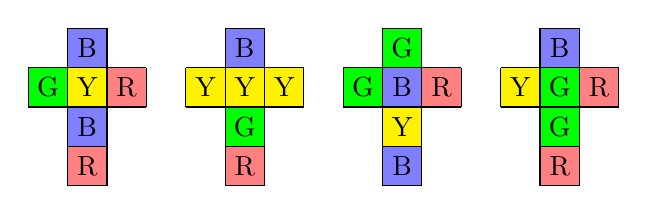
\begin{tikzpicture}[scale=.5]

\fill[red!50!white] (1,0) rectangle (2,1);
\fill[blue!50!white] (1,1) rectangle (2,2);
\fill[yellow] (1,2) rectangle (2,3);
\fill[blue!50!white] (1,3) rectangle (2,4);
\fill[green] (0,2) rectangle (1,3);
\fill[red!50!white] (2,2) rectangle (3,3);
\draw (1.5, .5) node {R};
\draw (2.5, 2.5) node {R};
\draw (1.5, 1.5) node {B};
\draw (1.5, 2.5) node {Y};
\draw (1.5, 3.5) node {B};
\draw (.5, 2.5) node {G};



\draw (1,0) grid (2,4);
\draw (0,2) grid (3,3);


\begin{scope}[xshift=4cm]

\fill[red!50!white] (1,0) rectangle (2,1);
\fill[green] (1,1) rectangle (2,2);

\fill[blue!50!white] (1,3) rectangle (2,4);
\fill[yellow] (0,2) rectangle (3,3);



\draw (1.5, .5) node {R};
\draw (1.5, 1.5) node {G};
\draw (1.5, 2.5) node {Y};
\draw (1.5, 3.5) node {B};
\draw (.5, 2.5) node {Y};
\draw (2.5, 2.5) node {Y};
\draw (1,0) grid (2,4);
\draw (0,2) grid (3,3);
\end{scope}

\begin{scope}[xshift=8cm]

\fill[blue!50!white] (1,0) rectangle (2,1);
\fill[yellow] (1,1) rectangle (2,2);
\fill[blue!50!white] (1,2) rectangle (2,3);
\fill[green] (1,3) rectangle (2,4);
\fill[green] (0,2) rectangle (1,3);
\fill[red!50!white] (2,2) rectangle (3,3);
\draw (1.5, .5) node {B};
\draw (1.5, 1.5) node {Y};
\draw (1.5, 2.5) node {B};
\draw (1.5, 3.5) node {G};
\draw (.5, 2.5) node {G};
\draw (2.5, 2.5) node {R};


\draw (1,0) grid (2,4);
\draw (0,2) grid (3,3);
\end{scope}


\begin{scope}[xshift=12cm]

\fill[red!50!white] (1,0) rectangle (2,1);
\fill[green] (1,1) rectangle (2,2);
\fill[green] (1,2) rectangle (2,3);
\fill[blue!50!white] (1,3) rectangle (2,4);
\fill[yellow] (0,2) rectangle (1,3);
\fill[red!50!white] (2,2) rectangle (3,3);
\draw (1.5, .5) node {R};
\draw (1.5, 1.5) node {G};
\draw (1.5, 2.5) node {G};
\draw (1.5, 3.5) node {B};
\draw (.5, 2.5) node {Y};
\draw (2.5, 2.5) node {R};


\draw (1,0) grid (2,4);
\draw (0,2) grid (3,3);
\end{scope}



\end{tikzpicture}


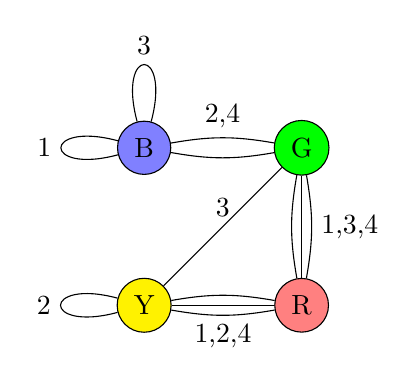
\begin{tikzpicture}[scale=2, every loop/.style={}, bend angle=10]


\node[fill=blue!50!white, draw=black, circle] (B) at (0,1) {B};
\node[fill=green, draw=black, circle] (G) at (1,1) {G};
\node[fill=red!50!white, draw=black, circle] (R) at (1,0) {R};
\node[fill=yellow, draw=black, circle] (Y) at (0,0) {Y};

\draw (B) edge[bend left] node[above] {2,4}(G)  ;
\draw (B) edge[bend right] (G)  ;

\draw (B) edge[loop left] node[left] {1} (B);
\draw (B) edge[loop above] node[above] {3} (B);
\draw (Y) edge node[above] {3} (G);
\draw (Y) edge[loop left] node[left] {2} (Y);
\draw (Y) edge[bend right] node[below] {1,2,4} (R);
\draw (Y) edge (R);
\draw (Y) edge[bend left] (R);
\draw (G) edge[bend left] node[right] {1,3,4} (R);
\draw (G) edge  (R);
\draw (G) edge[bend right]  (R);

\end{tikzpicture}



\end{document}
